\documentclass[floatfix,nofootinbib,superscriptaddress,fleqn]{revtex4}  
%\documentclass[aps,epsfig,tightlines,fleqn]{revtex4}
\usepackage[utf]{kotex}
\usepackage[HWP]{dhucs-interword}
\usepackage[dvips]{color}
\usepackage{graphicx}
\usepackage{bm}
%\usepackage{fancyhdr}
%\usepackage{dcolumn}
\usepackage{defcolor}
\usepackage{amsmath}
\usepackage{amsfonts}
\usepackage{amssymb}
\usepackage{amscd}
\usepackage{amsthm}
\usepackage[utf8]{inputenc}
 \usepackage{setspace}
%\pagestyle{fancy}

\begin{document}

\title{\Large 2022년 1학기 물리학 I: Quiz 21}
\author{김현철\footnote{Office: 5S-436D (면담시간 매주
    화요일-16:00$\sim$20:00)}} 
\email{hchkim@inha.ac.kr}
\author{Lee Hui-Jae} 
\email{hjlee6674@inha.edu}
\affiliation{Hadron Theory Group, Department of Physics,
Inha University, Incheon 22212, Republic of Korea }
\date{Spring semester, 2022}


\vspace{1.cm}

\maketitle

\vspace{1cm}
\noindent {\bf 문제 1. (100 pt)} 
103.0 kPa의 계기압력에서
$0.140\,\mathrm{m}^3$의 부피를 갖는 101.3 kPa의 압력까지 등온 팽창한
다음, 일정압력에서 처음부피가 될 때까지 냉각시켰다. 기체가 한 일을
계산하여라(계기압력은 실제압력과 대기압의 차이이다). 
 \vspace{1cm}
 
\noindent {\bf 풀이 : }
등온 팽창 과정에서
기체의 처음 부피, 압력, 온도를 $V_1$, $P_1$, $T_1$라 하고
기체의 나중 부피, 압력, 온도를 $V_2$, $P_2$, $T_1$라 하자. 
등온 팽창 과정을 먼저 살펴보자. 
등온 과정이므로 두 상태의 온도는 같고 문제에서 주어준 변수는
$P_1 = 103.0\,\mathrm{kPa}$, $V_2 = 0.140\,\mathrm{m^3}$
,$P_2 = 101.3\,\mathrm{kPa}$이다.
이상기체 상태방정식으로부터
\begin{align}\label{eq:1-1}
    & nRT_1=P_1V_1=P_2V_2
\end{align}
임을 알 수 있다.
등온 팽창 과정 중 기체가 한 일을 $W_1$이라 하면
\begin{align}
  dW_1 = PdV = \frac{nRT}{V}\,dV
\end{align}
이므로 등온 과정에 대해 적분하면 온도가 상수이므로 적분 밖으로 꺼낼 수 있고
\begin{align}
  W_1 = nRT_1\int^{V_2}_{V_1}\frac{1}{V}\,dV
  = P_2V_2 \ln\frac{V_2}{V_1}
\end{align}
이다. 식~\eqref{eq:1-1}로부터
\begin{align}
  W_1 =P_2V_2 \ln\frac{P_1}{P_2} 
\end{align}
라고 쓸 수 있다.
등온 팽창 과정 이후 등압 과정에서 기체의 나중 부피, 압력, 온도를 $V_1$, $P_2$, $T_3$라 하자.
처음 부피가 되었으므로 부피는 $V_1$이고 등압 과정이므로 압력은 $P_2$이다.
이 과정 중에 기체가 한 일 $W_2$는
\begin{align}
  W_2 = \int^{V_1}_{V_2}P_2\,dV = P_2(V_1-V_2)
\end{align}
이고 $V_1$을 주어진 변수들로 표현하면
\begin{align}
  W_2 = P_2\left(\frac{P_2V_2}{P_1}-V_2\right)
  =P_2V_2\left(\frac{P_2}{P_1}-1\right)
\end{align}
이다. 전체 과정 중에 기체가 한 일 $W$은
\begin{align}
  \begin{split}
    W=&W_1+W_2 =P_2V_2\left(\ln\frac{P_1}{P_2}+\frac{P_2}{P_1}-1\right) \\
    =&(101.3\,\mathrm{kPa})(0.140\,\mathrm{m^3})\left(
      \ln\frac{(103.0\,\mathrm{kPa})}{(101.3\,\mathrm{kPa})}
      +\frac{(101.3\,\mathrm{kPa})}{(103.0\,\mathrm{kPa})}-1\right) \\
     =& 0.00195\,\mathrm{kPa\cdot m^3} 
     =1.95\,\mathrm{J} 
  \end{split}
\end{align}
임을 얻는다.
\vspace{1cm}

\noindent {\bf 문제 2. (100 pt)}
$\gamma=1.30$인 기체가 처음 상태 273 
K, 1.00 atm에서 갑자기 처음부피의 절반으로 단열압축되었다.
\begin{itemize}
\item[(가)] 나중 압력과
\item[(나)] 나중 온도를 구하여라. 
\item[(다)] 그런 다음 기체가 일정한 압력에서 273 K까지 냉각되었다면,
  나중부피는 얼마인가?   
\end{itemize}
\vspace{1cm}
\noindent {\bf 풀이 : }
기체의 처음 부피, 압력, 온도를 $V_1$, $P_1$, $T_1$라 하고
기체의 나중 부피, 압력, 온도를 $V_2$, $P_2$, $T_2$라 하자. 
\begin{itemize}
  \item[(가)] 
단열과정이므로
\begin{align}\label{eq:2}
  P_1V_1^\gamma = P_2V_2^\gamma
\end{align}
를 만족하고 단열압축하여 처음부피의 절반이 되었다 하였으므로
\begin{align}\label{eq:2-1}
  V_2 = \frac{1}{2}V_1
\end{align} 
이다. 식~\eqref{eq:2-1}를 식~\eqref{eq:2}에 대입하여
\begin{align}\label{eq:2-2}
  P_1V_1^\gamma = P_2\left(\frac{1}{2}V_1\right)^\gamma  
  \Longrightarrow P_2 =2^\gamma P_1
\end{align}
를 얻는다. 계산해보면
\begin{align}
  P_2 = 2^{1.30}(1.00\,\mathrm{atm}) = 2.46\,\mathrm{atm}
\end{align}
이다.
  \item[(나)] 
  이상기체 상태방정식과 식~\eqref{eq:2-1},~\eqref{eq:2-2}으로부터
  \begin{align}\label{eq:2-3}
    T_2 = \frac{P_2V_2}{nR}
    =\frac{1}{nR}\left(2^{\gamma }P_1\right)\left(\frac{1}{2}V_1\right)
    =2^{\gamma-1}\frac{P_1V_1}{nR}
    =2^{\gamma-1}T_1
  \end{align}
  이므로
  \begin{align}
    \begin{split}
      T_2 = 2^{0.30}(273\,\mathrm{K}) = 336\,\mathrm{K}
    \end{split}
  \end{align}
  이다.
  \item[(다)]
  등압과정을 거친 후 기체의 나중 부피, 압력, 온도를 $V_3$, $P_2$, $T_1$이라 하자. 
  등압과정이므로 기체의 압력은 $P_2$로 일정하고 기체의 온도가 처음 상태와 같으므로 온도는
  $T_1$이다. 따라서
  \begin{align}
    P_2 = \frac{nRT_2}{V_2} = \frac{nRT_1}{V_3}
  \end{align}
  과 같이 쓸 수 있으며 식~\eqref{eq:2-1},~\eqref{eq:2-3}을 대입하면 나중부피 $V_3$을 얻을 수 있다.
  \begin{align}
    \begin{split}
      V_3 &= \frac{T_1}{T_2}V_2 = \frac{T_1}{2^{\gamma-1}T_1}\left(\frac{1}{2}V_1\right)
      =2^{-\gamma}V_1 \\
      &= 2^{-1.30}V_1 = 0.406V_1.
    \end{split}
  \end{align}
  \end{itemize}

\vspace{1cm}

\noindent {\bf 문제 3. (200pt)}
그림~\ref{fig:1}은 1.00 몰의 단원자
이상적인 기체의 순환과정이다.  각각의 과정에서 온도는 $T_1=400$ K,
$T_2=600$ K, $T_3=455$ K이다.  $1\to 2$ 과정에 대해
\begin{figure}[ht]
  \centering
  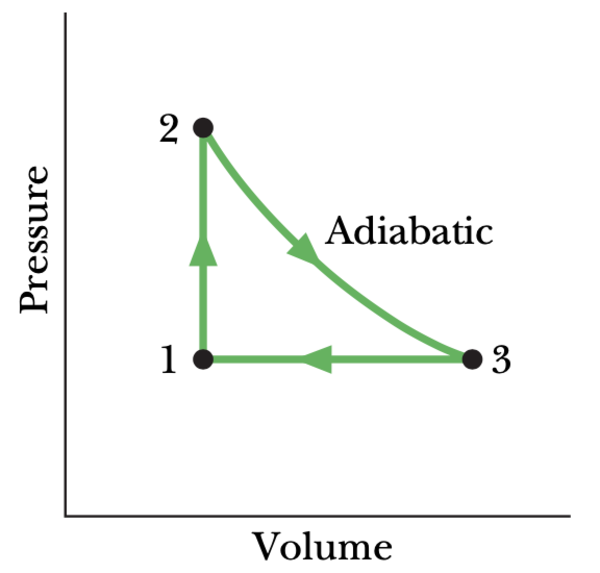
\includegraphics[scale=0.6]{Qfig23-1.pdf}
  \caption{문제 3}
  \label{fig:1}
\end{figure}
\begin{itemize}
\item[(가)] 열 $Q$
\item[(나)] 내부에너지 변화 $\Delta U$
\item[(다)] 한 일은 각각 얼마인가? 
\item[(라)] $2\to 3$과정에 대하여 $Q$
\item[(마)] $\Delta U$
\item[(바)] $W$는 각각 얼마인가? 
\item[(사)] $3\to 1$과정에서 
\item[(아)] $Q$
\item[(자)] $\Delta U$
\item[(차)] $W$는 얼마인가?
\item[(카)] 전체 순환 과정에 대해 $Q$
\item[(타)] $\Delta U$
\item[(파)] $W$는 각각 얼마인가?
\end{itemize}
점 1에서 처음 압력은 1.00 기압 ($=1.013\times 10^5$ Pa)이다. 점 2에서
\begin{itemize}
\item[(하)] 부피 
\item[(거)] 압력을 구하여라. 
\end{itemize}
점 3에서 
\begin{itemize}
\item[(너)] 부피 
\item[(더)] 압력을 구하여라. 
\end{itemize}
\vspace{1cm}
\noindent {\bf 풀이 : }

$1\to 2$ 과정은 등적과정이므로 열역학 제 1법칙에 의해
\begin{align}\label{eq:3-1}
  dU = dQ -PdV = dQ
\end{align}
라고 쓸 수 있다. 즉, 내부에너지 변화량 $dU$와 기체가 외부로부터 받는 열 $dQ$가 같다.
내부에너지 $U$는
\begin{align}\label{eq:3-2}
  U=\frac{3}{2}nRT
\end{align}
이므로 식~\eqref{eq:3-1}로부터
\begin{align}
  \Delta U_{1\to 2} = Q_{1\to 2} = \frac{3}{2}nR(T_2-T_1)
\end{align}
이다. 따라서 $1\to 2$ 과정에 대한
\begin{itemize}
  \item[(가)] 열 $Q_{1\to 2}$는
  \begin{align}
    \begin{split}
      Q_{1\to 2} &= \frac{3}{2}nR\left((600\,\mathrm{K})-(400\,\mathrm{K})\right)
      = \frac{3}{2}(8.314\,\mathrm{J\cdot K^{-1}})(200\,\mathrm{K}) \\
      &= 2490\,\mathrm{J}
    \end{split}
  \end{align}
  이다.
  \item[(나)] 
  내부에너지 변화량 $\Delta U _{1\to 2}$는 $Q_{1\to 2}$와 같으므로 2490 J이다.
  \item[(다)] 
  등압과정이므로 기체가 한 일은 0이다.
\end{itemize}
$2\to 3$ 과정은 단열과정이므로 $dQ=0$이고 열역학 제 1법칙에 의해
\begin{align}
  dU = -PdV = -dW
\end{align}
를 따른다. 식~\eqref{eq:3-2}로부터
\begin{align}
  \Delta U_{2\to 3} = \frac{3}{2}R(T_3-T_2)
\end{align}
이다. 따라서 $2\to 3$ 과정에 대한
  \begin{itemize}
  \item[(라)] 열 $Q_{2\to 3}$는 0이고
  \item[(마)] 내부에너지 변화량 $\Delta U_{2\to 3}$는
  \begin{align}
    \begin{split}
      \Delta U_{2\to 3} &= \frac{3}{2}(8.314\,\mathrm{J\cdot K^{-1}})
      ((455\,\mathrm{K})-(600\,\mathrm{K})) \\
      &= -1810\,\mathrm{J}
    \end{split}
  \end{align}
  이다.
  \item[(바)]
  기체가 한 일 $W_{2\to 3}$는 1810 J이다.
\end{itemize}
$3\to 1$ 과정은 등압과정이다. 열역학 제 1법칙에 의해
\begin{align}\label{eq:3-3}
  dU = dQ -dW
\end{align}
 이고 식~\eqref{eq:3-2}로부터
\begin{align}\label{eq:3-4}
  \Delta U_{3\to 1} = \frac{3}{2}R(T_1-T_3)
\end{align}
이다. 또한 기체가 한 일 $W_{3\to 1}$은
\begin{align}
  W_{3\to 1} = P_1\Delta V = P_1V_1-P_1V_3
\end{align}
인데 $P_1=P_3$이므로 $W_{3\to 1}$을 다음과 같이 쓸 수 있다.
\begin{align}\label{eq:3-5}
  W_{3\to 1} = P_1V_1-P_3V_3 = R(T_1-T_3).
\end{align}
식~\eqref{eq:3-3}에 의해 $Q_{3\to 1}$는
\begin{align}\label{eq:3-6}
  Q_{3\to 1} = \Delta U_{3\to 1} + W_{3\to 1}
  = \frac{5}{2}R(T_1-T_3)
\end{align}
이다.
  \begin{itemize}
  \item[(사)] 따라서 $2\to 3$ 과정에 대한
  \item[(아)] 열 $Q_{3\to 1}$은 식~\eqref{eq:3-6}에 의해
  \begin{align}
    \begin{split}
      Q_{3\to 1} &= \frac{5}{2}(8.314\,\mathrm{J\cdot K^{-1}})
      ((400\,\mathrm{K})-(455\,\mathrm{K})) \\
      &= -1140\,\mathrm{J}
    \end{split}
  \end{align} 
  이고
  \item[(자)] 내부에너지 변화량 $\Delta U_{3\to 1}$은 식~\eqref{eq:3-4}에 의해
  \begin{align}
    \begin{split}
      \Delta U_{3\to 1} &= \frac{3}{2}(8.314\,\mathrm{J\cdot K^{-1}})
      ((400\,\mathrm{K})-(455\,\mathrm{K})) \\
      &= -686\,\mathrm{J}
    \end{split}
  \end{align}
  이다.
  \item[(차)] 기체가 한 일 $W_{3\to 1} $ 은 식~\eqref{eq:3-5}에 의해
  \begin{align}
    \begin{split}
      W_{3\to 1} = &= (8.314\,\mathrm{J\cdot K^{-1}})
      ((400\,\mathrm{K})-(455\,\mathrm{K})) \\
      &= -457\,\mathrm{J}
    \end{split}
  \end{align}
  이다.
  \item[(카)] 
  전체 순환과정에 대한 열 $Q$는
  \begin{align}
    \begin{split}
      Q &= Q_{1\to 2}+Q_{2\to 3}+Q_{3\to 1}
      =\frac{3}{2}R(T_2-T_1)+0+\frac{5}{2}R(T_1-T_3) \\
      &= R\left(T_1 + \frac{3}{2}T_2 - \frac{5}{2}T_3\right)  \\
      &= (8.314\,\mathrm{J\cdot K^{-1}})
      \left((400\,\mathrm{K}) + \frac{3}{2}(600\,\mathrm{K}) 
      - \frac{5}{2}(455\,\mathrm{K})\right)  \\
      &=1350\,\mathrm{J}
    \end{split}
  \end{align}
  이고
  \item[(타)] 
  전체 순환과정에 대한 내부에너지 변화량 $\Delta U$는
  \begin{align}
    \begin{split}
      \Delta U &= \Delta U_{1\to 2}+ \Delta U_{2\to 3}+ \Delta U_{3\to 1} \\
      &= \frac{3}{2}R(T_2-T_1+T_3-T_2+T_1-T_3)  \\
      &= 0
    \end{split}
  \end{align}
  이다.
  \item[(파)] 전체 순환과정에 대한 일 $W$는
  \begin{align}
    \begin{split}
      W &= W_{1\to 2}+W_{2\to 3}+W_{3\to 1}
      =0+ \frac{3}{2}R(T_2-T_3) + R(T_1-T_3)  \\
      &= R\left(T_1 +\frac{3}{2}T_2 -\frac{5}{2}T_3\right)  \\
      &= (8.314\,\mathrm{J\cdot K^{-1}})
      \left((400\,\mathrm{K}) + \frac{3}{2}(600\,\mathrm{K}) 
      - \frac{5}{2}(455\,\mathrm{K})\right)  \\
      &=1350\,\mathrm{J}
    \end{split}
  \end{align}
  으로 전체 순환과정에 대한 열 $Q$와 같다.
\end{itemize}
$1\to 2$ 과정은 등적과정이므로 $V_1=V_2$이고 이상기체 상태방정식에 의해
\begin{align}
  P_1V_1 = RT_1 \Longrightarrow V_1 = R\frac{T_1}{P_1}
\end{align}
이다.
\begin{itemize}
  \item[(하)] 점 2에서의 부피 $V_2$는
  \begin{align}
    \begin{split}
      V_2 &= V_1 = R\frac{T_1}{P_1} = (8.026\,\mathrm{m^3\cdot atm \cdot K^{-1}})
      \frac{(600\,\mathrm{K})}{(1\,\mathrm{atm})} \\
      &= 482\,\mathrm{m^3}
    \end{split}
  \end{align}
  이고
  \item[(거)] 
  점 2에서의 압력 $P_2$는
  \begin{align}
    \begin{split}
      P_2 &= R\frac{T_2}{V_2}=P_1\frac{T_2}{T_1} 
      = (1\,\mathrm{atm})\frac{(600\,\mathrm{K})}{(400\,\mathrm{K})} \\
      &= 1.5\,\mathrm{atm}
    \end{split}
  \end{align}
  이다.
\end{itemize}
$3\to 1$ 과정은 등압과정이므로 $P_1=P_3$이다. 따라서,
\begin{itemize}
  \item[(너)] 점 3에서의 부피 $V_3$는
  \begin{align}
    P_3V_3 = RT_3 \Longrightarrow V_3 = R\frac{T_3}{P_1}
  \end{align}
  이므로
  \begin{align}
    V_3 = (8.026\,\mathrm{m^3\cdot atm \cdot K^{-1}})
    \frac{(455\,\mathrm{K})}{(1\,\mathrm{atm})} 
    = 3650\,\mathrm{m^3}
  \end{align}
  이고
  \item[(더)] 
  점 3에서의 압력 $P_3$는 $P_1$과 같으므로
  \begin{align}
    P_3 = 1\,\mathrm{atm}
  \end{align}
  이다.
  \end{itemize}



\vspace{1cm}

\end{document}